%=====================================================================
\section{Elastic theory of the wall layer: shielding}\label{sec:theory}
B.~Loewe's picture: defects of equal charge repel, opposite charges attract, the strongly anchored wall repels every defect, and an evenly
distributed wall layer shields the bulk from its charge. Here it is made quantitative for the passive (elastic) part of the problem.
Scripts: \texttt{reports/master/theory/shielding\_disk.wl} (Mathematica; results in \texttt{shielding\_disk\_results.txt}) and
\texttt{shielding\_ellipse.wl} (conformal map; \texttt{shielding\_ellipse\_results.txt}).

\subsection{Model}
One-constant Frank elasticity, director angle $\theta$, defects of charge $q_i$ at $z_i$. Use the field $\psi$ conjugate to $\theta$
($\nabla\psi=\hat z\times\nabla\theta$), for which defects are point sources, $\nabla^2\psi=2\pi\sum_iq_i\delta(z-z_i)$. Strong anchoring fixes
$\theta$ on the wall, so $\partial_s\theta$ is prescribed: a \emph{Neumann} condition for $\psi$, with flux density equal to the imposed winding per
length ($2\pi k/P$ for winding uniform in arclength). In a disk the Neumann Green's function has images \emph{of the same sign} at $R^2/\bar z$, and
\begin{equation}
\frac{E}{\pi K}=-\sum_{i\ne j}q_iq_j\ln|z_i-z_j|-\sum_{i,j}q_iq_j\ln|R^2-z_i\bar z_j|\qquad(\text{core energies dropped}).
\label{eq:Eel}
\end{equation}
Its pieces are the poster's terms, up to the poster's sign convention ($U=-E$): $-2\pi Kq_iq_j\ln|z_i-z_j|=-\frac\pi2K\ln r_{ij}$ for like $\pm\half$
(repulsion), and the self-image term $-\pi Kq_i^2\ln(R^2-r_i^2)=-\frac\pi4K\ln(R^2-r_i^2)$ (repulsion from the wall, because the image has the same
sign: bringing a defect to a strongly anchored wall costs energy). Equation~\eqref{eq:Eel} adds the cross-image terms.

\subsection{Shielding in a circle is exact}
For $N$ wall charges $q_w$ evenly spaced on a ring of radius $r_w$, the identity $\sum_j\ln|z-r_we^{2\pi ij/N}|=\ln|z^N-r_w^N|$ gives the energy of a
bulk charge $q_t$ at $z=re^{i\varphi}$:
\begin{equation}
\frac{V(z)}{\pi K}=\text{const}-2q_tq_w\Big[\ln\big|1-(r/r_w)^Ne^{iN\varphi}\big|+\ln\big|1-(rr_w/R^2)^Ne^{iN\varphi}\big|\Big]-q_t^2\ln(R^2-r^2).
\label{eq:ring}
\end{equation}
Both brackets vanish on angular average (for $a<1$, $\oint\ln|1-ae^{it}|\,dt=0$; checked numerically): \textbf{inside the ring the bulk does not feel
the wall layer at all, whatever its charge}, apart from a corrugation of relative size $(r/r_w)^N$ next to it. For 14 wall $-\half$ at $R=1.43\,\la$
the energy of a bulk $+\half$ varies by only $0.019\,\pi K$ over $r<0.7R$. This is the 2D shell theorem with images, and it explains why the bulk is
$+1$ for every $k$ (Sec.~\ref{sec:ccharge}): the overcharge is invisible from inside.

\subsection{Where the passive layer sits: a parameter-free check}
The energy of a passive ring of $N$ charges $q$ at radius $r$ is, from Eq.~\eqref{eq:Eel},
$E(r)/\pi K=-q^2N[(N-1)\ln r+\ln(R^{2N}-r^{2N})]+\text{const}$. Its minimum (verified symbolically: $dE/dr=0$, $d^2E/dr^2>0$) is
\begin{equation}
r^*=R\left(\frac{N-1}{3N-1}\right)^{1/2N},\qquad d=R-r^*\xrightarrow{N\to\infty}\frac{\ln3}{4\pi}\,\ell\approx0.087\,\ell,\qquad\ell=\frac{2\pi R}{N}.
\label{eq:depth}
\end{equation}
Like charges repel along the wall and all are repelled by it; the balance puts the ring at a depth proportional to the spacing. This is the passive
depth law found empirically in Sec.~\ref{sec:passive} ($\langle s\rangle\approx0.56+0.094/\rho$, with $1/\rho$ the spacing).
\begin{figure}[H]\centering
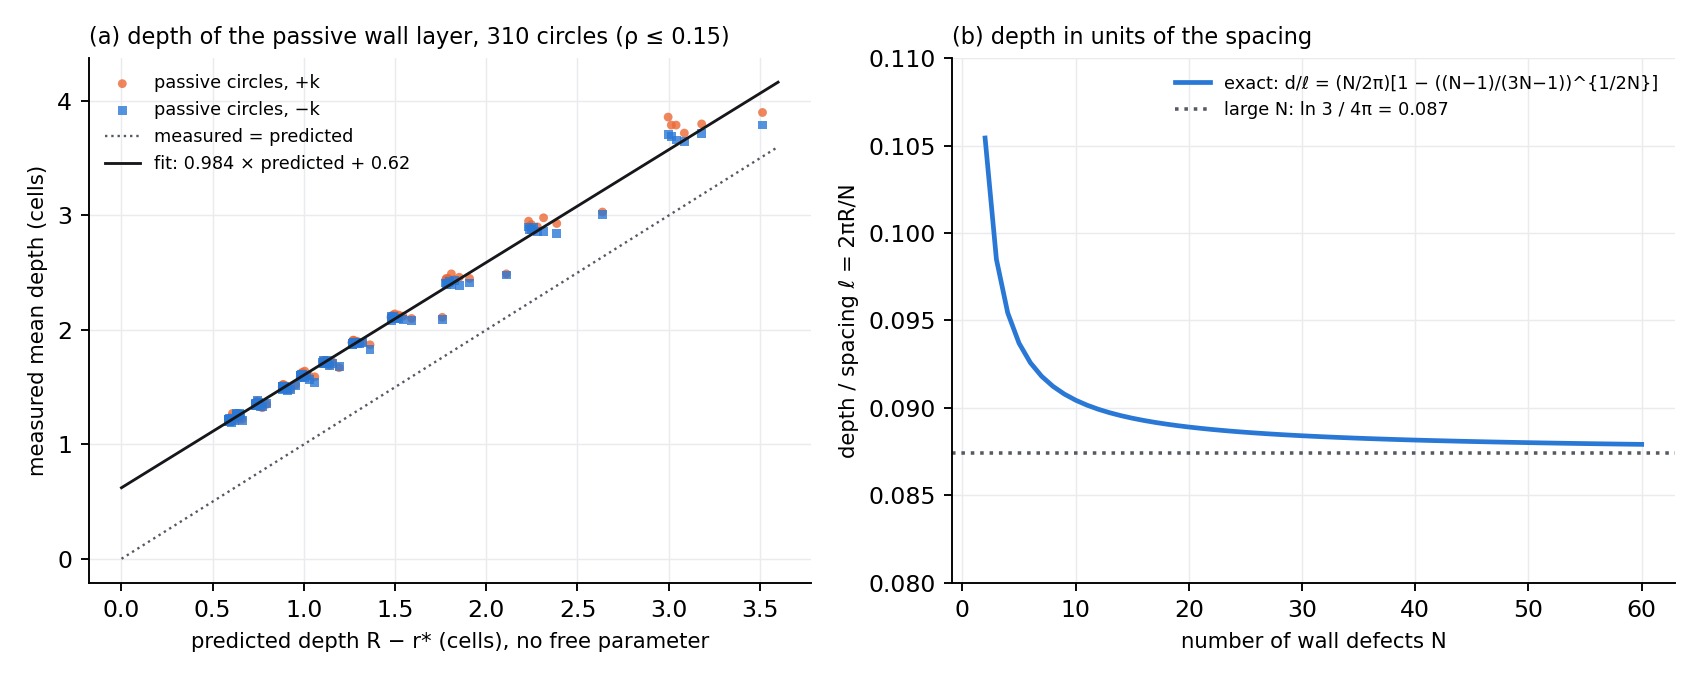
\includegraphics[width=\textwidth]{depth_law.png}
\caption{(a) Measured mean depth of the imposed defects in 310 passive circles ($\rho\le0.15$, both signs) against the parameter-free prediction of
Eq.~\eqref{eq:depth}: measured $=0.984\times$ predicted $+\,0.62$ cells, correlation 0.996. The offset (0.61 cells, IQR 0.60--0.62, the same for
both signs) is where the cell-based anchoring places the effective wall. (b) Depth in units of the spacing against $N$.}\label{fig:depthlaw}
\end{figure}
With a bulk charge $Q_b$ at the centre (the active layer) the minimum becomes $r^*=R[(N-1+2Q_b/q)/(3N-1+2Q_b/q)]^{1/2N}$ (verified), so a $+1$
bulk pushes the layer slightly closer to the wall.

\subsection{Approach of a bulk defect to the wall layer}
Equation~\eqref{eq:ring} along a radius gives the energy of a bulk $+\half$ approaching the $-\half$ wall layer of a mirror circle ($k=-6$,
$R=1.43\,\la$, 14 sites at the depth of Eq.~\eqref{eq:depth} plus the 0.61-cell offset), compared with a free $\pm\half$ pair.
\begin{figure}[H]\centering
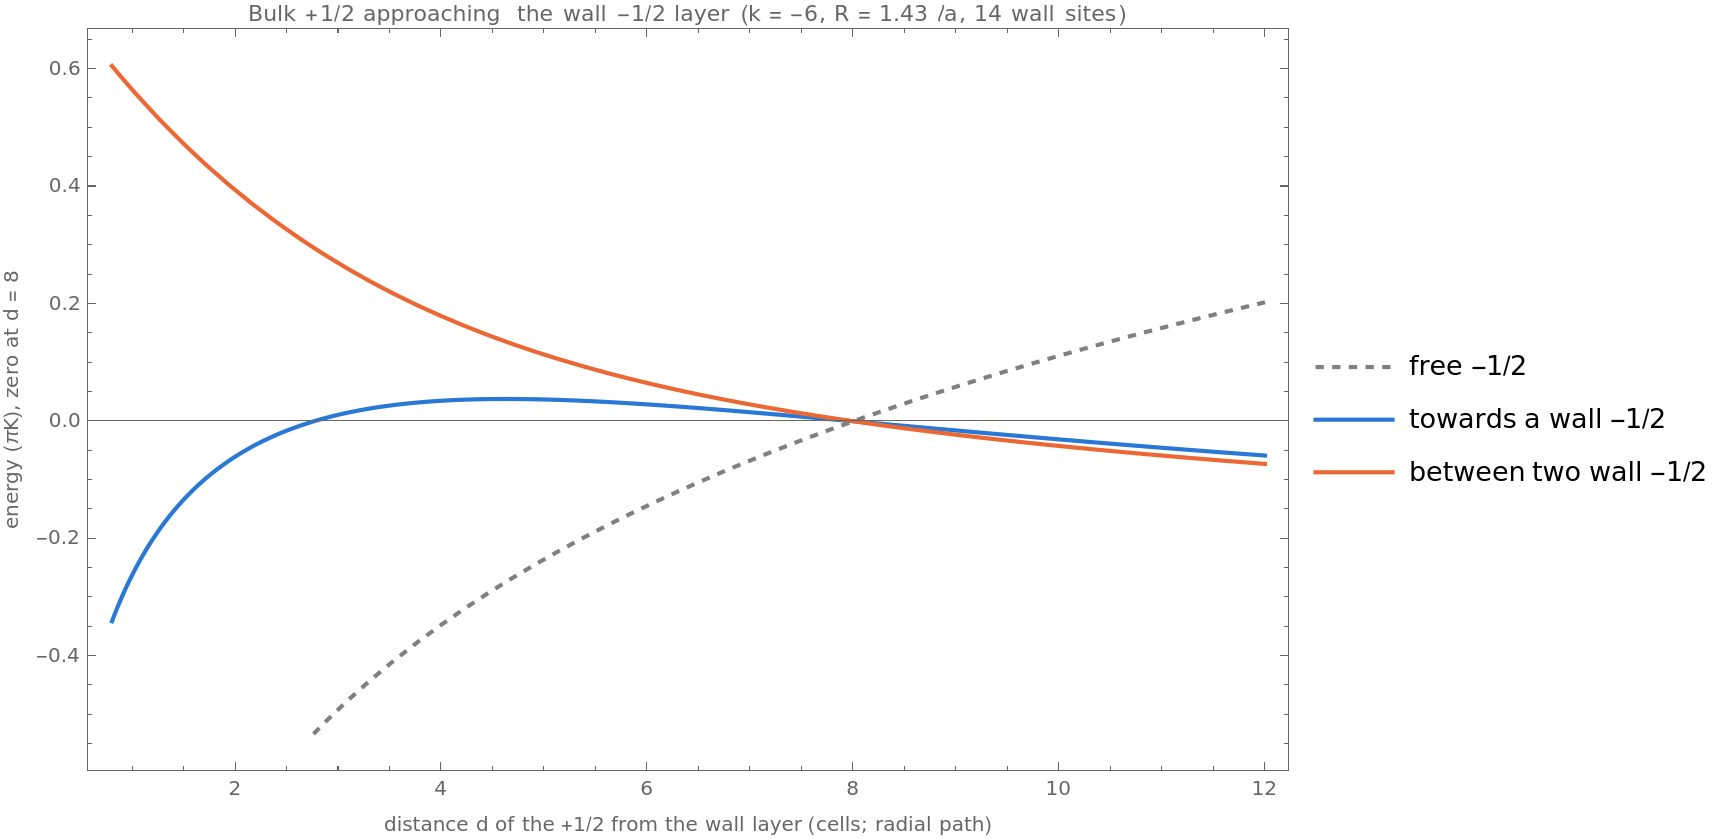
\includegraphics[width=0.85\textwidth]{approach_energy.png}
\caption{Energy of a bulk $+\half$ against its distance from the wall layer along a radius (zero at 8 cells): towards a wall $-\half$ (blue), towards
the gap between two wall $-\half$ (orange), and towards a free $-\half$ (dashed).}\label{fig:approach}
\end{figure}
\begin{table}[H]\centering\small
\caption{Energy released (in $\pi K$) as the $+\half$ moves inwards, theory, and the measured counterpart (shielding test, Sec.~\ref{sec:shield}).}\label{tab:approach}
\begin{tabular}{lccc}\toprule
& towards a free $-\half$ & towards a wall $-\half$ & ratio\\\midrule
theory, from 8 to 4 cells & 0.35 & $-0.03$ (small barrier) & --\\
theory, from 4 to 1 cell & 0.69 & 0.30 & 0.43\\
simulation: encounters reaching $\le2$ cells & 57\% & 28\% & 0.49\\
simulation: encounters ending in annihilation & 53\% & 22\% & 0.41\\\bottomrule
\end{tabular}
\end{table}
The layer turns the long-range attraction into a short-range one: towards a wall $-\half$ there is a small barrier ($\approx0.04\,\pi K$ at 4--5
cells) and attraction only within $\approx3$ cells, with less than half the energy gain of a free pair; towards the gap between two wall defects the
bulk $+\half$ is repelled all the way ($+0.6\,\pi K$ at contact). The measured suppression sits, as predicted, mostly in the approach.

\subsection{Ellipses: shielding is imperfect but the leftover field is weak}
For an ellipse with winding uniform in arclength (eMode 2) the conformal map $w(z)=m^{1/4}\,\mathrm{sn}\!\big(\tfrac{2K(m)}{\pi}\arcsin\tfrac zc,m\big)$
($c^2=A^2-B^2$, nome $((A-B)/(A+B))^2$) sends the cavity to the unit disk. The Neumann Green's function with uniform flux is
$G(z,\zeta)=\ln|w-\omega|+\ln|1-w\bar\omega|+H(z)+H(\zeta)$, where $H$ is harmonic with $\partial_nH=2\pi/P-|w'(z)|$ on the wall (a smooth
boundary datum, solved by a Fourier series). Checks: $|w|=1$ on the wall to $10^{-13}$; for $\varepsilon\to1$ the relaxed ring depth (1.33 cells)
equals Eq.~\eqref{eq:depth} (1.328). Twelve passive $+\half$ were relaxed (from two ring orientations; equal energies), then a bulk test charge
was placed inside.
\begin{table}[H]\centering\small
\caption{Ellipses of area 2500 with 12 $+\half$ ($k=6$), passive equilibrium. Spacing: density ratio flank gap/tip gap (uniform 1, conductor
$\varepsilon$). Shielding: range of the energy that the wall layer (with its images and the boundary winding) gives a bulk $+\half$, inside the
0.6 and 0.8 levels, and centre minus tip regions.}\label{tab:ellth}
\begin{tabular}{lcccc}\toprule
& circle & $\varepsilon=1.2$ & $\varepsilon=1.5$ & $\varepsilon=2.0$\\\midrule
relaxed depth (cells) & 1.33 & 1.33--1.35 & 1.35--1.39 & 1.42--1.55\\
spacing, density ratio (theory / passive simulation) & 1.00 / -- & 1.00 / 0.97 & 1.01 / 0.98 & 1.01 / 0.98\\
layer energy range, inside 0.6 level ($\pi K$) & 0.003 & 0.008 & 0.021 & 0.059\\
layer energy range, inside 0.8 level ($\pi K$) & 0.12 & 0.15 & 0.22 & 0.33\\
centre minus tip regions ($\pi K$) & 0.003 & $-0.002$ & $-0.010$ & $-0.019$\\\bottomrule
\end{tabular}
\end{table}
\begin{itemize}
  \item The passive layer stays evenly spaced in arclength (theory and simulation agree); it does not adopt the screening (conductor) distribution.
  \item The shielding of an ellipse is therefore imperfect: the leftover field in the inner part grows $\approx20\times$ from the circle to
        $\varepsilon=2$. It stays an order of magnitude below the approach energies near the wall ($\lesssim0.06\,\pi K\approx6\,k_BT$ in the inner 60\%, pushing a
        bulk $+\half$ slightly towards the centre), but is not negligible compared with $k_BT$ (Sec.~\ref{sec:frank}).
  \item \textbf{Consequence:} elastic shielding explains the circle (the bulk is blind to $k$; the passive depth; the screened approach), but the
        unscreened elastic field in an ellipse is probably too weak to destroy the layer on its own. The loss of the layer in elongated cavities is more
        likely driven by the flow: two vortices instead of one, wandering and escaping wall defects, depleted tips (Secs.~\ref{sec:slattice},
        \ref{sec:sflow}). The negative-winding ellipses (running) test this: $-\half$ are not self-propelled.
\end{itemize}
\subsection{Energy scale: the Frank constant of the MPCD nematic}\label{sec:frank}
The Frank constants are not inputs of nematic MPCD; they were measured from the equilibrium director fluctuations of a passive, defect-free,
periodic $64\times64$ box (two seeds; size check $96\times96$, one seed) with the cavity parameters (density 20, mean-field potential $U=10\,k_BT$, collision operator 21 at zero activity),
initially aligned along $x$: for a director along $x$, $Ak_BT/\langle|\theta_{\mathbf q}|^2\rangle=K_1q_y^2+K_3q_x^2$, fitted over $|q|<0.8$ with a
constant for the cell-level noise (\texttt{runs/Kcalib/frank\_constant.py}, 900 frames per run, $\langle S\rangle=0.876$, no defects; the mean director stays within $16^\circ$ of $x$
in every frame). The spectrum is linear in $q^2$ along both axes, with splay stiffer than bend at every wavenumber (Fig.~\ref{fig:frank}); single modes
scatter by up to $12\,k_BT$ at $q<0.3$ (one mode each), which the two-constant fit averages.
\begin{table}[H]\centering\small
\caption{Frank constants of the 2D MPCD nematic ($U=10\,k_BT$, density 20; $k_BT$; seeds 1, 2: $64\times64$). \texttt{reports/master/data/frank\_constants.txt}.}\label{tab:frank}
\begin{tabular}{lccc}\toprule
& $K_1$ (splay) & $K_3$ (bend) & one-constant $K=(K_1+K_3)/2$\\\midrule
seed 1 & 42.1 & 22.6 & 32.4\\
seed 2 & 41.9 & 23.5 & 32.7\\
$96\times96$, seed 1 & 41.5 & 23.0 & 32.3\\\bottomrule
\end{tabular}
\end{table}
\begin{figure}[H]\centering
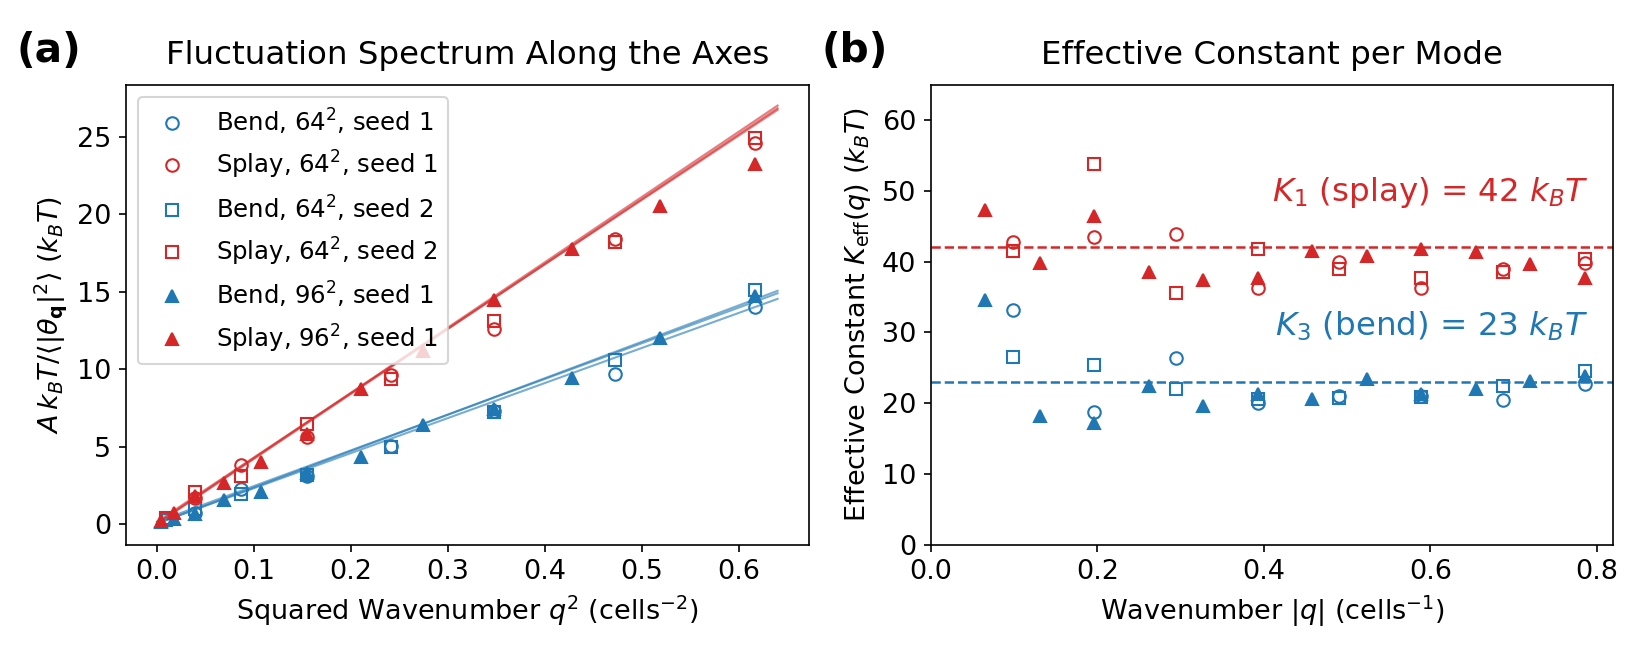
\includegraphics[width=\textwidth]{frank_spectrum.png}
\caption{Director fluctuations of the passive periodic boxes ($U=10\,k_BT$, density 20, director along $x$). (a) Inverse mode amplitude
$A\,k_BT/\langle|\theta_{\mathbf q}|^2\rangle$ ($A$ the box area) against $q^2$ along the bend ($q_x$, blue) and splay ($q_y$, red) axes; lines: the
two-constant fit $K_1q_y^2+K_3q_x^2+c$ of each box over $|q|<0.8$ ($c$ the white noise of the cell estimate). (b) Effective constant of each mode,
$K_\mathrm{eff}=A\,k_BT/(q^2\langle|\theta_{\mathbf q}|^2\rangle)$; dashed: $K_1=42$ and $K_3=23\,k_BT$. Open symbols $64\times64$ (circles seed 1,
squares seed 2), filled triangles $96\times96$. \texttt{scripts/fig\_frank.py}; \texttt{data/frank\_constants.txt}.}\label{fig:frank}
\end{figure}
In 2D the elasticity is not isotropic (splay $\approx1.8\times$ bend; in 3D the original algorithm paper reports isotropic constants,
$K_i\approx113\,U$ per unit length (T.~N.~Shendruk and J.~M.~Yeomans, Soft Matter \textbf{11}, 5101 (2015))). With $K\approx32\,k_BT$, $\pi K\approx100\,k_BT$: the approach barrier towards a wall
$-\half$ is $\approx4\,k_BT$, the pull from 4 to 1 cell $\approx30\,k_BT$ (free pair $\approx70$), the repulsion between two wall defects $\approx60\,k_BT$,
and the leftover field inside an $\varepsilon=2$ ellipse $\approx6\,k_BT$ in the inner 60\% and $\approx33\,k_BT$ inside the 0.8 level (circle: $0.3$).
Near the wall the shielding energies are tens of $k_BT$, so thermal noise plays no role and activity moves the defects; whether the leftover field in
an ellipse is weak has to be judged against the active driving, not against $k_BT$. \emph{Activity in the same units} (from the code of collision operator 21): each particle in a cell is kicked by $\pm\zeta N_\mathrm{cell}\cdot\half\cdot\Delta t$
along the director, opposite on the two sides of a plane through the centre of mass (sigmoid factor $\half$ at the mean density), i.e.\ a force of
$\approx0.7$ per particle and a force dipole of $\approx3.5$ per cell: an active stress $\zeta_\mathrm{eff}Q$ with $\zeta_\mathrm{eff}\approx4$, not the bare
$\zeta=0.07$. Then $\sqrt{K/\zeta_\mathrm{eff}}\approx2.8$ cells and $\la\approx8\sqrt{K/\zeta_\mathrm{eff}}$, the usual ratio in continuum simulations.
(An earlier version compared $\sqrt{K/\zeta}$ with the bare $\zeta$; that agreement was a coincidence.)

\subsection{Hydrodynamics: Stokes model of the defect forces}\label{sec:hydro}
\noindent\fbox{\parbox{0.97\textwidth}{\textbf{Correction (2026-10-07): sign error in this subsection and in Sec.~\ref{sec:fluct} (stage 2).}
The defect angle written by the code is the direction of $\nabla\!\cdot Q$ (\texttt{topoAngleLocal}), which for a $+\half$ points to its
\emph{tail} (splay side). Free bulk $+\half$ move \emph{against} this angle (mean step $-0.56$ to $-0.70$ cells per 2 time units, 66--72\% of steps,
$\approx60\sigma$; \texttt{theory/fluct/pinning/head\_convention.py}), as expected for extensile activity: the head, the self-propulsion and the active
force on the fluid all point along $-\hat e_\psi$. All $+\half$ forces below were placed along $+\hat e_\psi$. Consequences:
(i) wall $+\half$ have their tails at the wall and their heads pointing into the bulk, leaning \emph{upstream} (consistent with the upstream drift of
wall defects); their own active forces \emph{oppose} the circulation. The large variance explained by the wall term reflects the tilt being locked to the
flow, not the wall layer driving it; with physical signs a non-negative fit gives the wall layer zero weight. (ii) Bulk $+\half$ drive the circulation
(correlation $+0.5$ in circles) but, as point forces, explain only 6--21\% of the flow variance and do not predict the vortex number in ellipses.
(iii) In the feedback analysis the force reverses, so the wall layer \emph{damps} all tilt patterns, the one-vortex pattern most. Statements below that
the wall layer sustains the circulation are withdrawn pending a model built on the full active force $-\zeta_\mathrm{eff}\nabla\!\cdot Q$ of the
measured director field.}}

\emph{Idea (B.~Loewe):} treat the defects as point forces in a Stokes fluid with no-slip walls, their strength set by the activity. A $+\half$
exerts a net force along its axis, $\mathbf F=\zeta_\mathrm{eff}\!\int\!\nabla\!\cdot\!Q\,dA=\pi\zeta_\mathrm{eff}S\rho_\mathrm{cut}\,\hat{\mathbf e}$
(for an ideal $+\half$, $\nabla\!\cdot\!Q=S/(2r)$ along its axis, $\rho_\mathrm{cut}$ the size of its distorted region); a $-\half$ exerts no net force and
is modelled as three inward forces at $120^\circ$ (a force tripole, as in Norton et al.). Solved with finite elements in Mathematica (velocity and pressure,
no-slip disk, forces smeared over $\sigma=1.5$ cells; \texttt{reports/master/theory/stokes\_circle.wl}, \texttt{stokes\_frames/}).
\begin{figure}[H]\centering
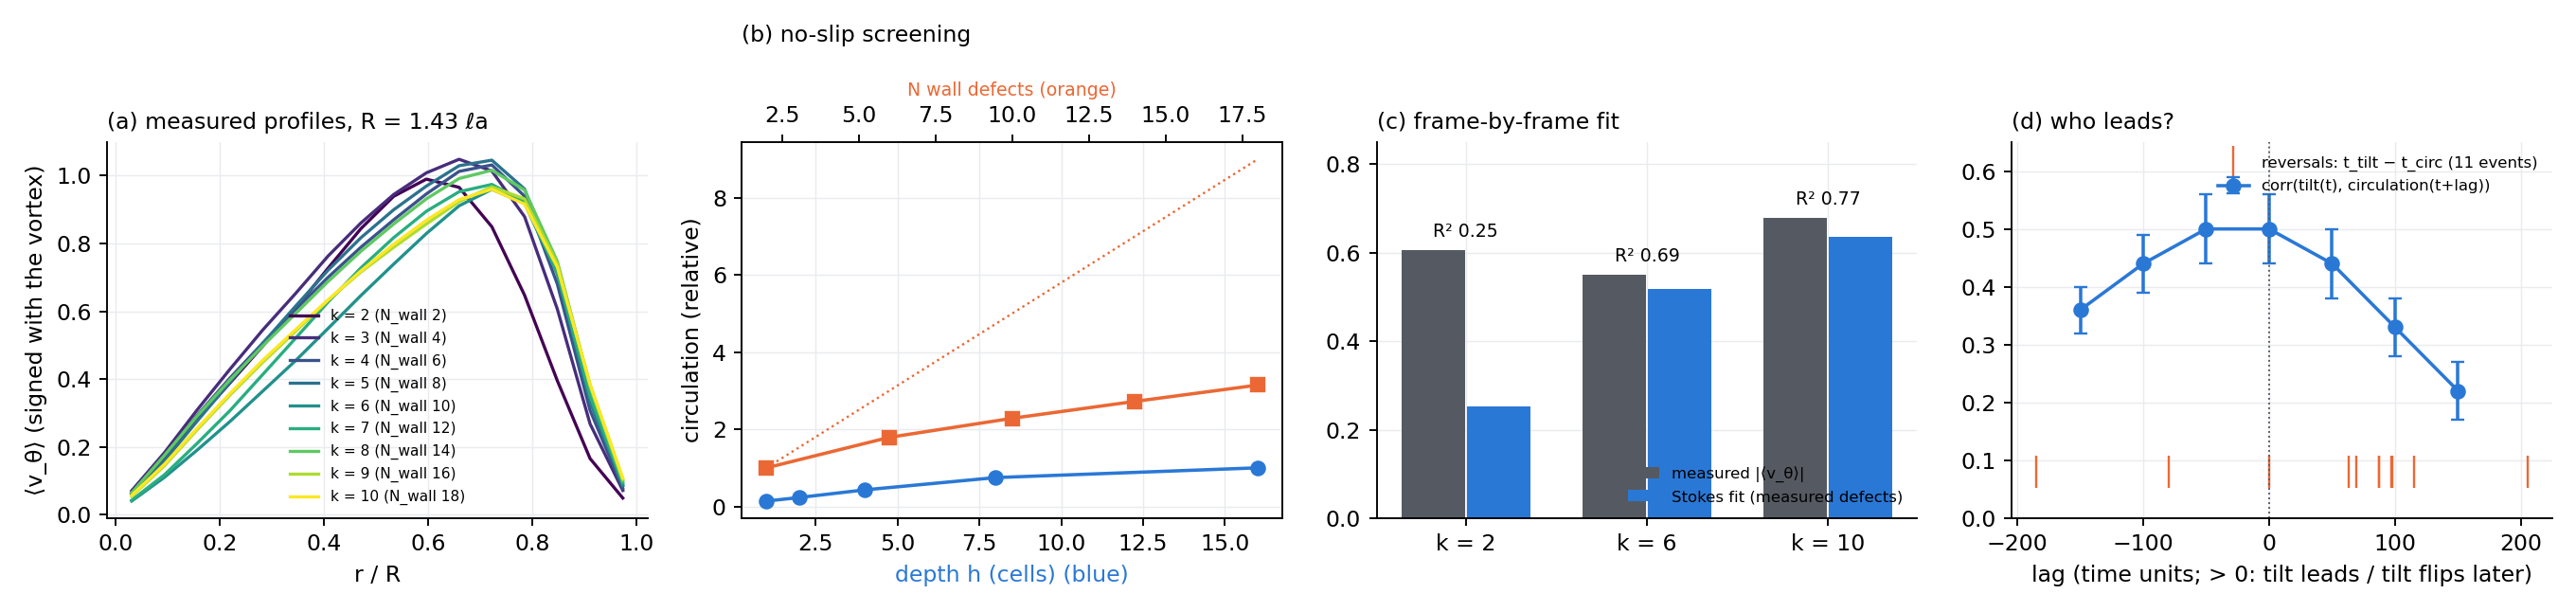
\includegraphics[width=\textwidth]{hydro_circle.png}
\caption{\textbf{Hydrodynamics of the wall layer in circles} ($R=1.43\,\la$). (a) Measured azimuthal velocity profiles for $k=2\dots10$ (fixed-radius scan,
seeds 2--3): the vortex is the same for 2 to 18 wall defects. (b) Static Stokes model: circulation driven by one tangential force against its depth
from the no-slip wall (blue, bottom axis), and by a wall layer of $N$ tilted $+\half$ at the predicted depths (orange, top axis; dotted: proportional to $N$);
both relative. (c) Circulation of the measured flow and of the Stokes flow of the measured defects (frame-by-frame fit), with the fraction of the
flow-field variance explained. (d) Timing: cross-correlation of the fluctuations of wall tilt and circulation (blue; lag $>0$: tilt leads), and the
delay of the tilt reversal after the circulation reversal at 11 vortex reversals ($\zeta=0.05$; orange ticks; $>0$: tilt flips later).}\label{fig:hydro}
\end{figure}
\begin{figure}[H]\centering
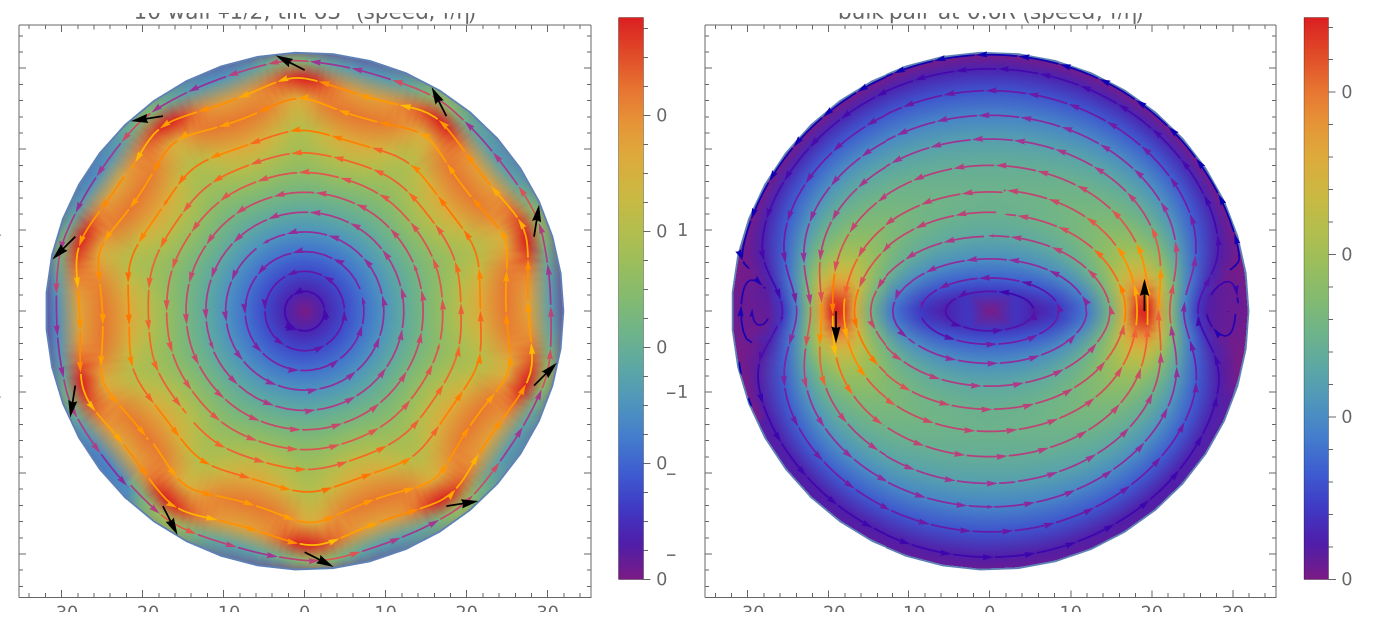
\includegraphics[width=0.85\textwidth]{stokes_circle_fields.png}
\caption{Static Stokes flows (speed in units of $f/\eta$): 10 wall $+\half$ tilted by $63^\circ$ (left) and a bulk pair of co-rotating $+\half$ at $0.6R$
(right).}\label{fig:stokesfields}
\end{figure}
\begin{itemize}
  \item \textbf{No-slip screening.} A force 1--2 cells from the wall drives 5--7$\times$ less circulation than one deep inside. Adding wall defects
        also pulls the layer closer to the wall (depth 5 $\to$ 1.5 cells for $N=2\to18$), so 9$\times$ more wall defects give only 3$\times$ more
        circulation (Fig.~\ref{fig:hydro}b). The $-\half$ tripoles produce essentially no circulation.
  \item \textbf{Measured flow, measured defects.} For each 50-time-unit flow interval the measured defects (every 5th defect frame) were turned into
        forces and the measured velocity field was regressed on the Stokes flows of the wall $+\half$, bulk $+\half$ and $-\half$. At $k=6$ and 10 the
        wall layer alone explains 67\% and 76\% of the flow field, the bulk $+\half$ 8\%, the tripoles nothing; the model circulation is 0.52 and 0.64
        against 0.55 and 0.68 measured. At $k=2$ the model fails (25\% explained, circulation 0.25 against 0.61). The fitted bulk coefficient is negative
        (not understood).
  \item \textbf{The force is of the right size.} The fitted force per wall defect is $f/\eta=20$, 11.5, 9.5 for $k=2$, 6, 10. With the active stress of
        collision operator 21, $\zeta_\mathrm{eff}\approx4$ (Sec.~\ref{sec:frank}), and the MPCD viscosity $\eta\approx17$ (2D formulas for density 20,
        $\Delta t=0.1$: kinetic 1.1, collisional 15.8), this means $\rho_\mathrm{cut}\approx31$, 18, 15 cells: between half the defect spacing and the cavity
        radius, shrinking as the wall gets crowded. The weaker push of a crowded layer, together with the screening, keeps the circulation independent of $k$.
  \item \textbf{But the vortex leads in time.} Fluctuations of wall tilt and circulation move together within one flow interval, with a slight asymmetry
        towards the circulation changing first (correlation 0.36 at $-150$ against 0.22 at $+150$ time units). At 11 vortex reversals (activity 0.05,
        $k=8$--10) the circulation flipped first in 9, the tilt following by a median of $\approx90$ time units.
  \item \textbf{Reading: two-way coupling.} The vortex sets the wall tilt; once tilted, the wall layer's active forces sustain most of the circulation.
        Reversals start elsewhere (the bulk). In an elongated cavity, once the flow organises into two vortices the wall layer loses the coherent tilt
        that sustains a single vortex (Part~III).
\end{itemize}
\paragraph{Ellipses.} \emph{Static:} a coherently tilted wall layer (10 $+\half$ evenly spaced in arclength at depth 1.5, all tilted $63^\circ$ the same way)
drives a \emph{single} vortex in every ellipse of area 2500: both halves rotate the same way, and the whole-cavity rotation drops only from 0.050 (circle)
to 0.033 $f/\eta$ ($\varepsilon=2$) (Fig.~\ref{fig:stokesell}). Elongation alone does not split the flow driven by the layer.
\begin{figure}[H]\centering
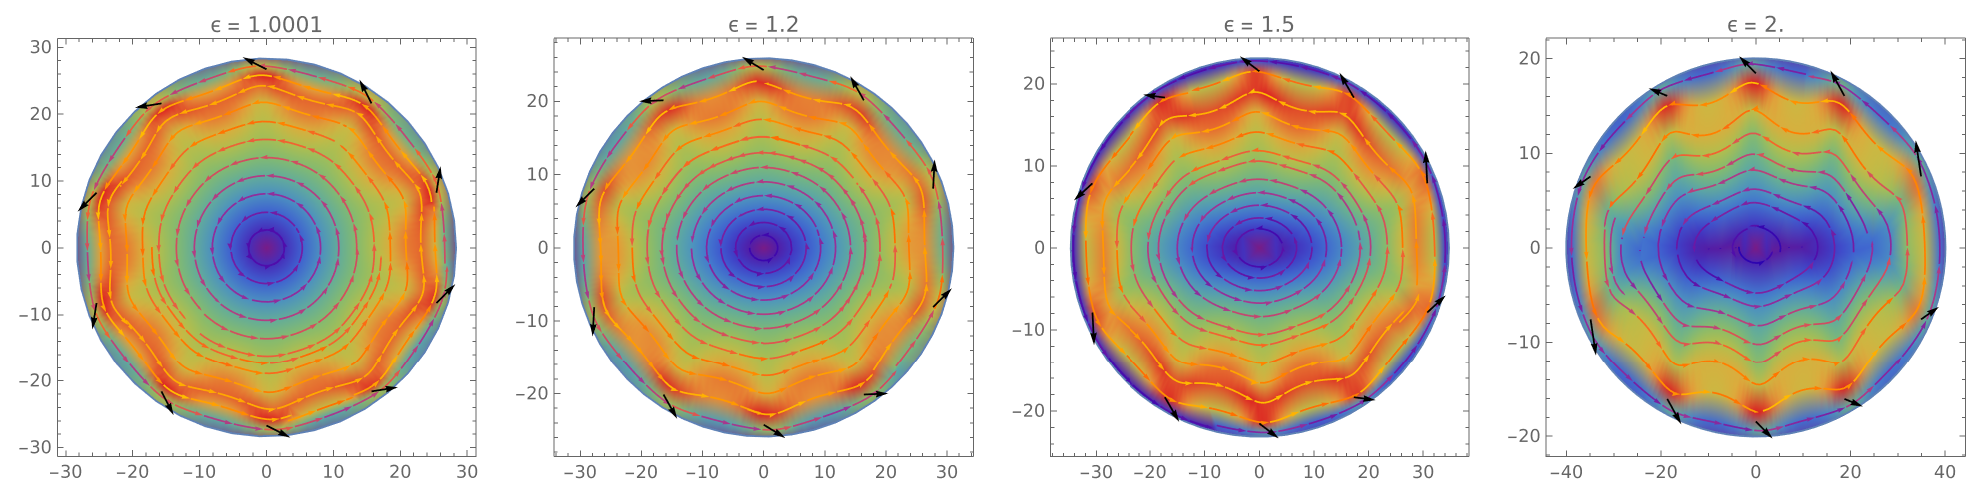
\includegraphics[width=\textwidth]{stokes_ellipse_static.png}
\caption{Stokes flow (speed, $f/\eta$) of a coherently tilted wall layer in a circle and ellipses $\varepsilon=1.2$, 1.5, 2.0 of the same area: a single vortex in all.}\label{fig:stokesell}
\end{figure}
\noindent\emph{Measured defects} (positive-winding ellipses, seed 1, 40 flow intervals of 100 time units each, same fit as for circles):
\begin{table}[H]\centering\small
\caption{Ellipses: Stokes fit of the measured flow on the forces of the measured defects. Half-cavity rotation: mean azimuthal velocity about the centroid of
each half; correlation over time between model and measurement.}\label{tab:hydroell}
\begin{adjustbox}{max width=\textwidth}
\begin{tabular}{lccc}\toprule
& $\varepsilon=1.2$ & $\varepsilon=1.5$ & $\varepsilon=2.0$\\\midrule
measured: halves rotating the same way & 100\% & 28\% & 45\%\\
measured: whole-cavity rotation & 0.57 & 0.26 & 0.09\\
flow variance explained: all / wall $+\half$ only / bulk $+\half$ only & 0.72 / 0.70 / 0.21 & 0.45 / 0.39 / 0.06 & 0.34 / 0.23 / 0.11\\
fitted $f/\eta$ per wall defect & 10.0 & 9.5 & 7.6\\
half-rotation, correlation model--measured (left / right) & 0.25 / 0.43 & 0.94 / 0.94 & 0.85 / 0.86\\
model: halves rotating the same way & 100\% & 40\% & 55\%\\\bottomrule
\end{tabular}
\end{adjustbox}
\end{table}
\begin{itemize}
  \item The measured wall defects reproduce the two-vortex dynamics of the elongated ellipses (half-rotation correlation 0.85--0.94, counter-rotation about
        right): their tilts follow the local vortex, and their forces reinforce the two-vortex flow.
  \item Since a coherently tilted layer would drive a single vortex, the two-vortex state is not imposed by the layer; it comes from the bulk, and the
        wall tilts follow, as the timing test in circles indicates.
  \item The wall layer matters less as the cavity elongates: it explains 70\% of the flow at $\varepsilon=1.2$ and 23\% at $\varepsilon=2.0$, while
        defects leave the wall and the bulk drives more of the flow. One seed per shape; the bulk coefficient is again negative.
\end{itemize}
\noindent\emph{Non-uniform tilts} (\texttt{theory/stokes\_tilt\_modes.wl}; same layer, 10 $+\half$ at depth 1.5, area 2500).
\begin{table}[H]\centering\small
\caption{Static Stokes flow of the wall layer with two tilt patterns: coherent (all $+63^\circ$) and split (left half $+63^\circ$, right half $-63^\circ$).
Rotation (units $f/\eta$) about the centroid of the left half, the right half and the whole cavity. At $\varepsilon=1.5$ one defect sits at $x\approx0$ and is
assigned to one half, hence the asymmetry.}\label{tab:tiltsplit}
\begin{tabular}{lccc}\toprule
$\varepsilon$ & coherent: left / right / whole & split: left / right / whole & split/coherent per half\\\midrule
1.0 & 0.039 / 0.039 / 0.050 & 0.026 / $-0.026$ / 0.000 & 0.68\\
1.2 & 0.040 / 0.040 / 0.048 & 0.029 / $-0.029$ / 0.000 & 0.73\\
1.5 & 0.038 / 0.038 / 0.043 & 0.036 / $-0.027$ / 0.013 & 0.83\\
2.0 & 0.032 / 0.032 / 0.033 & 0.030 / $-0.030$ / 0.000 & 0.94\\\bottomrule
\end{tabular}
\end{table}
\noindent\emph{Feedback modes.} Let $M_{ij}$ be the tangential velocity at wall defect $i$ due to a unit tangential force at wall defect $j$ (symmetric by
Stokes reciprocity). If tilts follow the local tangential flow and the tangential force follows the tilt, $M$ is the linear feedback operator of the
layer; its eigenvectors are the self-reinforcing tilt patterns and the eigenvalues their gains.
\begin{table}[H]\centering\small
\caption{Top eigenvalues of $M$ ($1/\eta$) and their mode type: uniform (all tilts the same, one vortex) or dipolar (left and right halves opposite, two vortices).
In the circle the dipolar mode is degenerate with its rotated partner ($m=1$ pair).}\label{tab:tiltmodes}
\begin{tabular}{lcccc}\toprule
$\varepsilon$ & uniform (1st) & dipolar (2nd) & ratio 1st/2nd & 3rd\\\midrule
1.0 & 0.0737 & 0.0653 & 1.13 & 0.0590\\
1.2 & 0.0735 & 0.0660 & 1.11 & 0.0645\\
1.35 & 0.0733 & 0.0663 & 1.11 & 0.0639\\
1.5 & 0.0730 & 0.0666 & 1.10 & 0.0633\\
1.65 & 0.0726 & 0.0668 & 1.09 & 0.0627\\
1.8 & 0.0722 & 0.0669 & 1.08 & 0.0621\\
2.0 & 0.0717 & 0.0670 & 1.07 & 0.0622\\
2.5 & 0.0705 & 0.0672 & 1.05 & 0.0637\\\bottomrule
\end{tabular}
\end{table}
\begin{itemize}
  \item \textbf{The layer can sustain two vortices.} A split layer drives two counter-rotating vortices with no net rotation, and the price of splitting
        disappears with elongation: per half, the split layer drives 68\% of the coherent rotation in the circle and 94\% at $\varepsilon=2$.
  \item \textbf{But it does not choose them.} The uniform (one-vortex) mode has the largest gain at every aspect ratio up to 2.5, so the wall
        hydrodynamics alone, in the linear feedback picture, would always select one vortex. The dipolar (two-vortex) mode is second from $\varepsilon=1.2$
        on, and its margin shrinks from 13\% (circle) to 5\% ($\varepsilon=2.5$): elongation makes the two states nearly degenerate.
  \item \textbf{Reading.} With nearly degenerate wall modes, a small push from the bulk is enough to select the two-vortex state, and the wall tilts then
        follow and reinforce it. This agrees with the timing in circles (the vortex leads) and with the falling wall share of the flow in ellipses
        (Table~\ref{tab:hydroell}). Measured tilt coherence: 1.00 (circle), 0.98--0.99 ($\varepsilon=1.2$), 0.43 ($\varepsilon=1.5$), 0.34 ($\varepsilon=2.0$).
  \item Caveats: linear, wall layer only, sites evenly spaced and fixed, tangential force only, no noise or elastic torque on the tilt.
\end{itemize}


\paragraph{Limits.} One-constant elasticity; orientation-dependent interactions ignored (the poster notes that they matter at the wall); core
energies and the cell scale enter only through the empirical 0.61-cell offset; no activity or flow. The energy scale $\pi K$ has not yet been
calibrated against the MPCD nematic parameters.
